\section{Task and EvidencePath Design}
\label{sec:method}
\subsection{Query, candidate, and target semantics}
A query $q=(c,m)$ pairs a cancer label with a CIViC molecular profile (MP) identifier. Frozen normalization defines each single drug $d$. Records retain evidence-item and source identifiers but contribute one $(q,d)$ evaluation pair. Distinct profiles remain distinct targets.

Graph pool $R_0(q)$ and evidence pool $E(q)$ give lists $L_g(q)$ and $L_e(q)$. Their union is $R_1(q)=R_0(q)\cup E(q)$, with additions $N(q)=E(q)\setminus R_0(q)$ and shared members $S(q)=R_0(q)\cap E(q)$. An empty graph branch does not remove a query from evaluation.

The endpoint set $P(q)$ includes all eligible positives, including drugs outside $R_1$. A therapy and blank-interaction screen precedes frozen single-drug adjudication, excluding generic classes and combinations. Positives require accepted predictive evidence supporting sensitivity/response at level A--D. We exclude pairs with both A/B support for sensitivity/response and A/B support for resistance or non-support for sensitivity/response. This eligibility rule is independent of the ranking conflict flag. Targets are annotations, not patient treatment outcomes.

\subsection{Source orders and membership control}
Figure~\ref{fig:framework} outlines the workflow. D1--D4 and ranks are illustrative; \emph{new} denotes evidence-exclusive candidates relative to $R_0$, and recall denotes positive-pair coverage.
\begin{figure}[t]
\centering
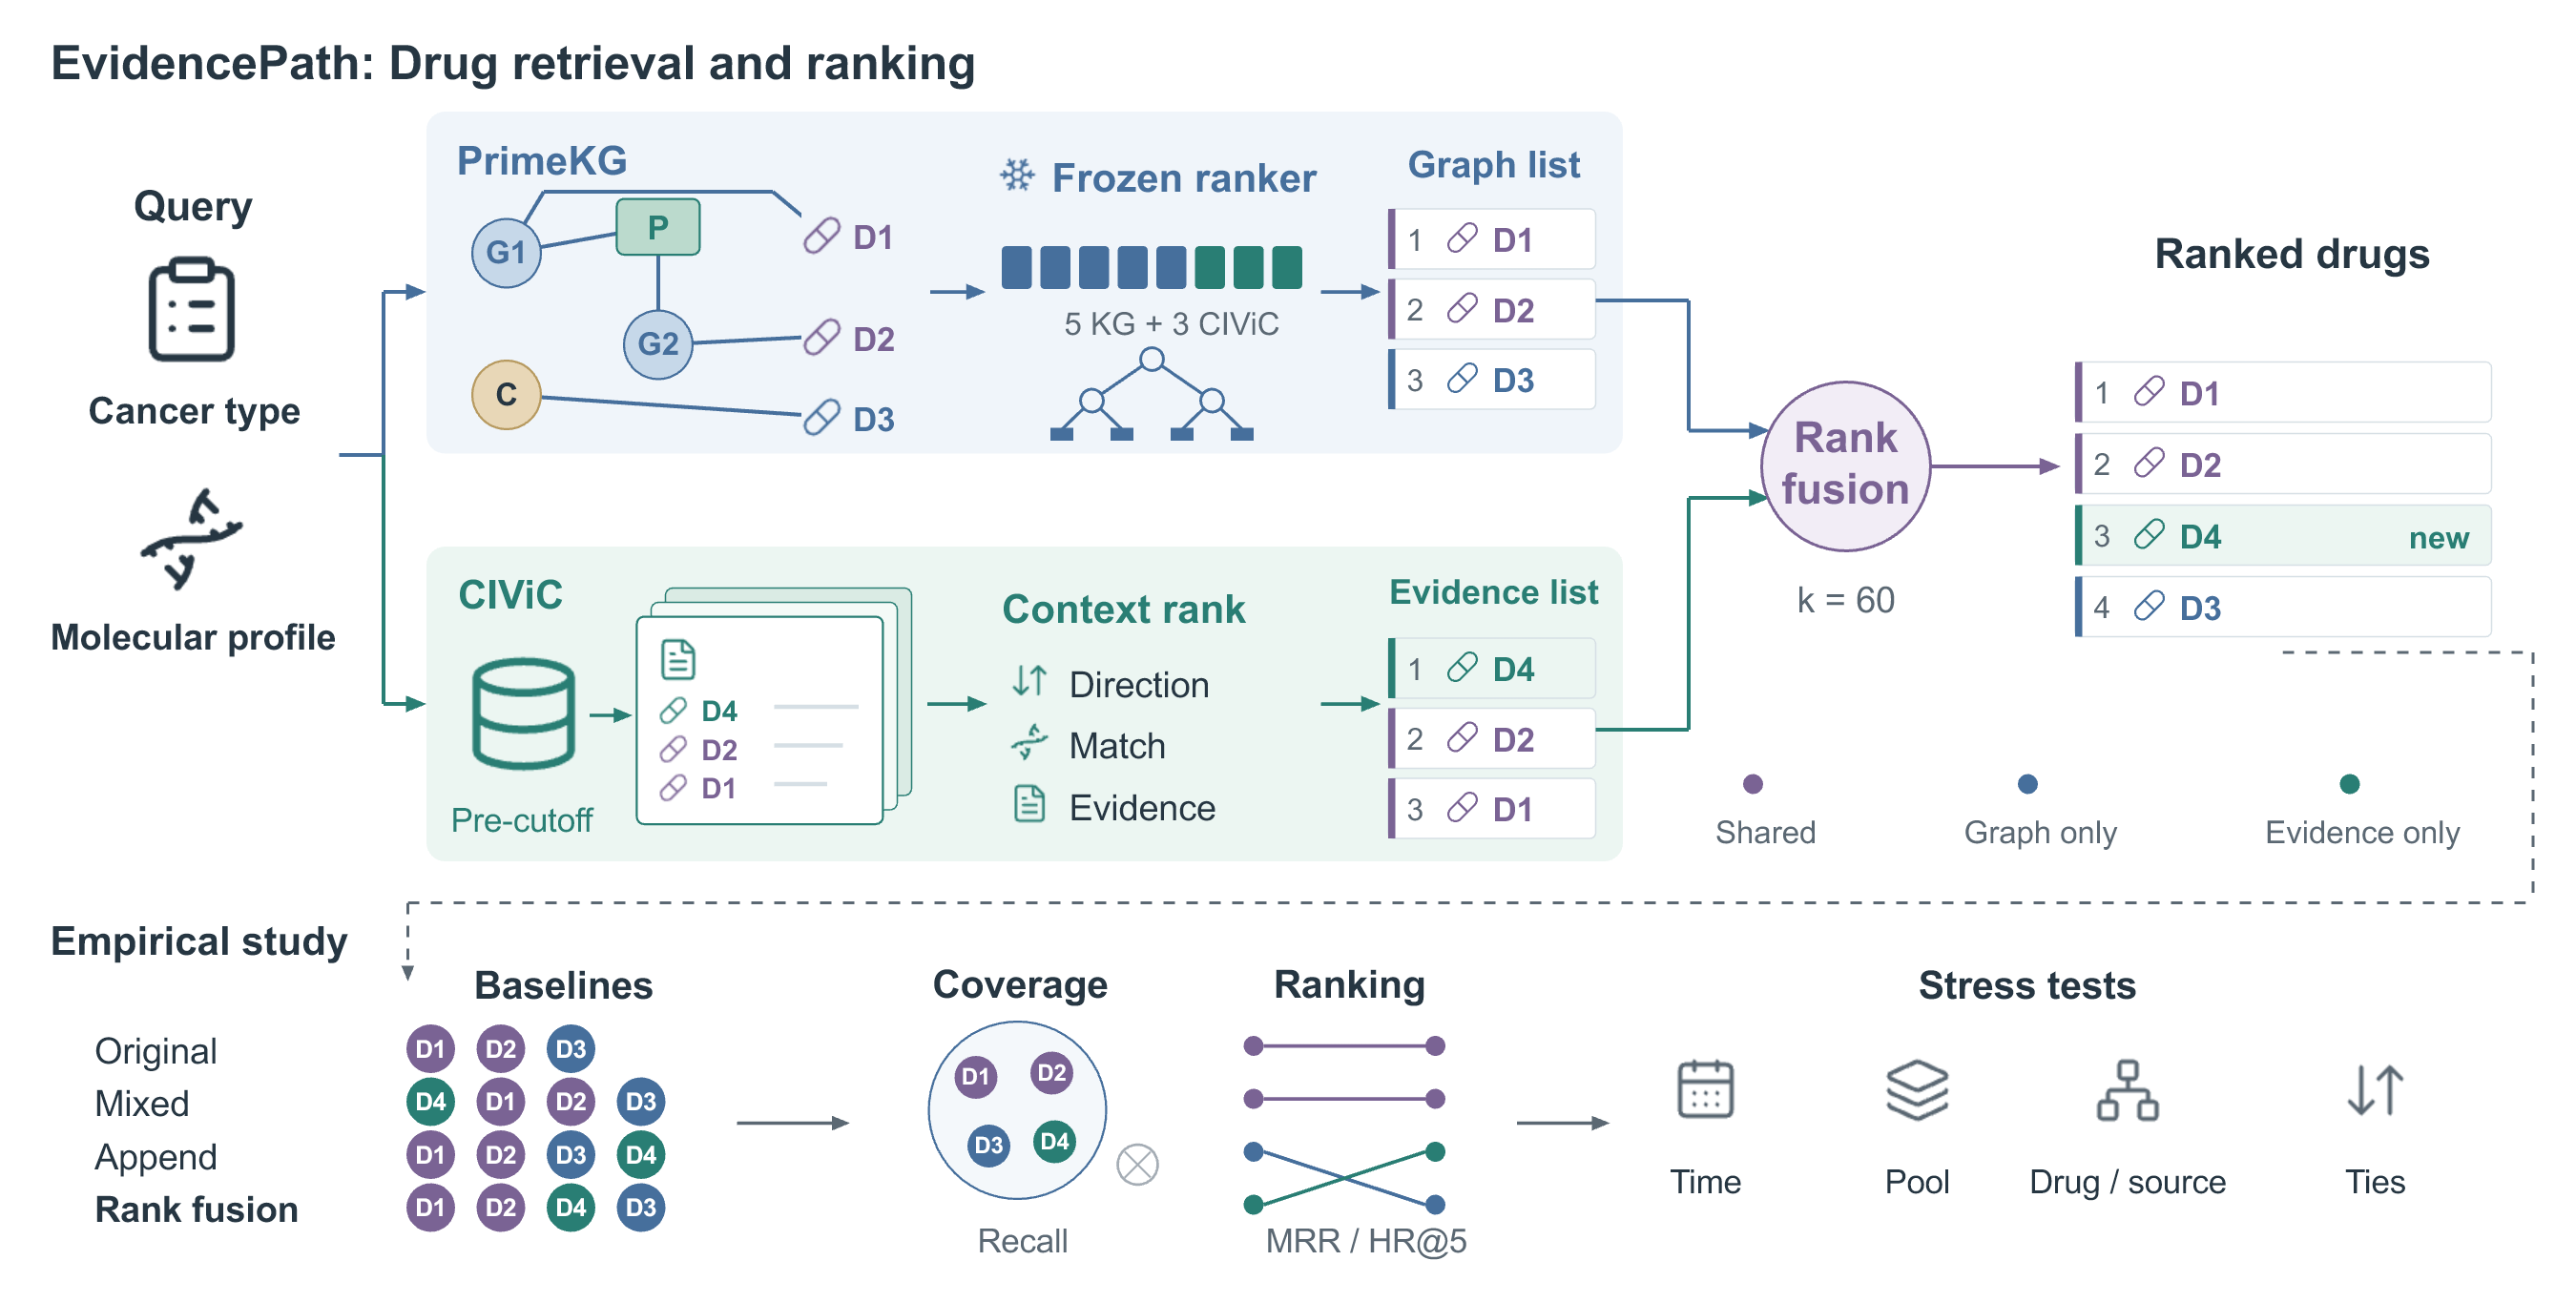
\includegraphics[width=\textwidth]{evidencepath-framework.png}
\caption{Workflow}
\label{fig:framework}
\end{figure}
\paragraph{Graph retrieval and frozen scoring.}
The graph branch unions direct targets, indications, and top-30 shared-pathway candidates (Table~\ref{tab:settings}).

SF is a frozen LightGBM LambdaMART ranker using graph and drug-level CIViC evidence (Table~\ref{tab:settings}). It scores the union once. The graph list restricts those scores to $R_0$, sorting by decreasing score then ascending canonical name. Graph names a pool, not a graph-feature-only scorer.

\paragraph{Clinical retrieval and order.}
Cutoff CIViC retrieval links identical profiles or shared validated genes in accepted predictive single-drug records, without an additional list truncation. Support for sensitivity/response is benefit; support for resistance, reduced sensitivity or adverse response is adversity. Non-support for sensitivity/response is anti-benefit. Other combinations are undetermined.

The descending key $(b,m,c,h,\ell,n,f)$ precedes ascending name. Benefit sets $b=2$, only opposition sets $b=0$, otherwise $b=1$. In tier 2, the best benefit maximizes $(m,c,\ell)$. Profile rank $m$ is 2 for identity or 1 for a shared gene. Disease rank $c$ is 2 for normalized equality, 1 for another known disease, or 0 for generic/missing disease. Levels A--E map to 5--1. Conflict sets $h=0$ if opposition has profile rank at least $m$, regardless of disease or level, otherwise $h=1$; the tier remains intact. Distinct benefit sources give $n$, SF gives $f$, and unused fields are zero. In tier 0, $\ell$ is the negative level of opposition selected by $(m,c,\ell)$.

\paragraph{Aggregation and control.}
For one-based source ranks, standard RRF is
\begin{equation}
s_{\mathrm{RRF}}(q,d)=\sum_{b\in\{g,e\}:\,d\in L_b(q)}\frac{1}{k+r_b(q,d)},\qquad k=60.
\label{eq:rrf}
\end{equation}
Each present branch contributes one equal-weight term. We compare rational scores exactly and break ties by name. Shared members receive two terms, exclusive members one. Length-normalized Borda sums $(|L_b|-r_b+1)/|L_b|$ over present lists and assigns zero for absence, using double precision and the same final tie rule. Aslam and Montague distribute remaining points to unranked items~\cite{metasearch}.

Context applies the full key to $R_1$. The parameter-free \emph{Shared-first} control stably places $S(q)$ before $R_1(q)\setminus S(q)$ in that full Context order. It preserves candidates, labels and within-block Context order, and is a post hoc diagnostic, not a validated new default.

\subsection{Separating coverage from displacement}
\label{sec:decomposition}
Let $\rr_M(q,d)=1/r_M(q,d)$ for a retrieved drug and zero otherwise, and $u_M(q)=\max_{d\in P(q)}\rr_M(q,d)$. Graph ranks $R_0$ and Mix ranks $R_1$ using the same frozen scores. Append-SF concatenates $O=L_g$ with SF-ordered additions $N_{\mathrm{SF}}$. Define $u_{\mathrm{Mix},0}$ at full Mix positions, maximizing only over $P(q)\cap R_0(q)$, or zero for an empty set. Then
\begin{align}
u_{\mathrm{Mix}}(q)-u_{\mathrm{Graph}}(q)
={}&\underbrace{u_{\mathrm{Mix},0}(q)-u_{\mathrm{Graph}}(q)}_{\text{original-positive displacement}}\nonumber\\
&+\underbrace{u_{\mathrm{Mix}}(q)-u_{\mathrm{Mix},0}(q)}_{\text{newly accessible-positive increment}}.
\label{eq:decomposition}
\end{align}
Both means use the same queries. With unchanged original scores and ties, Mix keeps the relative $R_0$ order, so the first term is nonpositive; the second is nonnegative. Append-SF fixes original absolute positions. We check these conditions against scores and historical exports.

\subsection{A limit of merging two fixed sequences}
\label{sec:bound}
Aslam and Montague's oracle follows unanimous pairwise preferences~\cite{metasearch}. Our conditional oracle preserves every within-list precedence of disjoint $O$ and $N_e$, the evidence-exclusive additions in $L_e$ order. If their first positive positions are $i^*,j^*$, or infinity when absent, the best merge attains
\begin{equation}
u_{\mathrm{2seq}}^*(q)=\max\left\{\frac{1}{i^*(q)},\frac{1}{j^*(q)}\right\},\qquad 1/\infty=0.
\label{eq:bound}
\end{equation}
Each positive follows its within-sequence predecessors; placing the sequence with the earlier first positive first attains the bound. Averaging bounds merges of these specified sequences. An old-order oracle fixes only $O$ and frees additions. Exceeding the two-sequence bound requires relaxing at least one constraint, not necessarily the graph order.
